\documentclass[11pt,a4paper]{article}

% ---------- Encoding & Language ----------
\usepackage[utf8]{inputenc}
\usepackage[T1]{fontenc}
\usepackage[english]{babel}

% ---------- Mathematics ----------
\usepackage{amsmath,amssymb,amsthm,mathtools}

% ---------- Page Layout & Typography ----------
\usepackage[margin=1.1in]{geometry}
\usepackage[protrusion=true,expansion=false]{microtype}
\usepackage{parskip}
\setlength{\parindent}{0pt}

% ---------- Graphics & Diagrams ----------
\usepackage{tikz}
\usetikzlibrary{arrows.meta, positioning, shapes.geometric, fit, calc, shadows.blur}
\usepackage{graphicx}

% ---------- Code & Verbatim ----------
\usepackage{listings}
\usepackage{xcolor}

\definecolor{codebg}{RGB}{248,248,245}
\definecolor{codekw}{RGB}{136,0,85}
\definecolor{codestr}{RGB}{34,119,34}
\definecolor{codecm}{RGB}{120,120,120}
\definecolor{accent}{RGB}{45,75,130}

\lstdefinelanguage{http}{
  morekeywords={GET,POST,PUT,DELETE,HTTP},
  keywordstyle=\color{codekw}\bfseries,
  sensitive=true,
}

\lstset{
  basicstyle=\ttfamily\small,
  backgroundcolor=\color{codebg},
  keywordstyle=\color{codekw}\bfseries,
  stringstyle=\color{codestr},
  commentstyle=\color{codecm}\itshape,
  frame=single,
  rulecolor=\color{gray!40},
  framesep=6pt,
  breaklines=true,
  showstringspaces=false,
  columns=fullflexible,
  xleftmargin=0.5em,
}

% ---------- Tables ----------
\usepackage{booktabs}
\usepackage{array}

% ---------- Hyperlinks ----------
\usepackage{hyperref}
\hypersetup{
  colorlinks=true,
  linkcolor=accent,
  urlcolor=accent,
  citecolor=accent,
}

% ---------- Epigraphs ----------
\usepackage{epigraph}
\setlength{\epigraphwidth}{0.72\textwidth}
\renewcommand{\textflush}{flushright}
\renewcommand{\epigraphflush}{flushright}
\renewcommand{\epigraphsize}{\small\itshape}

% ---------- Theorem-like Environments ----------
\theoremstyle{definition}
\newtheorem{definition}{Definition}[section]
\newtheorem{example}[definition]{Example}

\theoremstyle{remark}
\newtheorem*{remark}{Remark}
\newtheorem*{aside}{Aside}

% ---------- Title ----------
\title{\textbf{Networking, Web Services, and Inference APIs} \\[0.4em]
       \large Lecture Notes on TCP/IP, HTTP, gRPC, and Observability}
\author{Lecture Transcript --- Edited and Typeset}
\date{}

\begin{document}
\maketitle


\begin{abstract}
\noindent
These notes accompany a hybrid lecture--seminar on the practical deployment of modern web services. We begin with the theoretical foundations of the TCP/IP suite and the Hypertext Transfer Protocol, proceed to the deployment of a simple inference service with Flask, survey observability through Prometheus and Grafana, and conclude with a treatment of gRPC and Protocol Buffers as the workhorse protocols of inter-service communication. Throughout, the emphasis is on the \emph{why} behind each design decision: why reliability costs overhead, why human-readable formats yield to binary ones at service boundaries, and why geography quietly shapes the architecture of distributed systems.
\end{abstract}

\tableofcontents
\vspace{1em}\hrule\vspace{1em}

% ============================================================
\section{Orientation and Agenda}

Today's session is conducted in a hybrid format: a lecture component develops the theoretical scaffolding, and a seminar component grounds that scaffolding in running code. The sequence is deliberate; the abstractions are easier to love once one has seen them misbehave.

\paragraph{Plan of the lecture.}
We will treat, in order, the following topics:
\begin{itemize}
    \item the TCP/IP protocol suite and the HTTP protocol;
    \item deployment of a simple classification service using the Flask micro-framework;
    \item metrics collection with Prometheus and visualization with Grafana;
    \item gRPC and Protocol Buffers, with an eye toward microservice communication.
\end{itemize}

\paragraph{Homework assignments.}
To consolidate these themes, three assignments accompany the lecture.
\begin{enumerate}
    \item \textbf{Package management and testing.} Wrap your existing code into a \texttt{uv} package and write a \texttt{pytest} suite achieving high coverage.
    \item \textbf{ML classifier service.} Implement a machine learning classifier exposing both an HTTP and a gRPC interface.
    \item \textbf{Monitoring.} Integrate Prometheus to scrape the classifier's runtime metrics.
\end{enumerate}

\begin{remark}
gRPC is \emph{not} a replacement for HTTP. It is a high-performance alternative used predominantly for internal communication between backend services, where its efficiency and ergonomics make it the de facto choice for stitching microservices together.
\end{remark}

% ============================================================
\section{The TCP/IP Protocol Suite}


Networking is an irreducibly complex endeavour. To manage the complexity, we decompose it into layers, each responsible for a narrow concern and each communicating only with its immediate neighbours. Data descends the stack at the sender, is transmitted along the physical medium, and ascends a symmetric stack at the receiver. Although the OSI model is more commonly discussed in textbooks, the working engineer lives inside its leaner cousin, the four-layer TCP/IP model.

\subsection{The Four Layers}

\begin{description}
    \item[Application Layer.] The layer in closest contact with the user. It specifies the semantics of the conversation: \textsc{http} and \textsc{https} for web content, \textsc{smtp} for mail, \textsc{ssh} for remote shells, and so on.

    \item[Transport Layer.] Responsible for end-to-end communication between processes. Two protocols dominate: \textsc{tcp}, which is connection-oriented and reliable, and \textsc{udp}, which is connectionless and favours speed over guarantees. \textsc{udp} is used where a missed packet is cheaper than a delayed one---video streaming, voice over IP, \textsc{dns} lookups.

    \item[Internet Layer.] Concerned with \emph{logical} addressing and routing. The Internet Protocol (IP, in its v4 and v6 incarnations) identifies hosts uniquely; routers, operating at this layer, determine which path a packet takes through the network.

    \item[Network Interface Layer.] The physical substrate. Ethernet cables, Wi-Fi adapters, network cards, and the electrical or optical signals that carry bits. Ohm's law lives here; so, nowadays, do fibre optics and InfiniBand, the latter displacing copper in high-performance environments where bandwidth and latency budgets are tight.
\end{description}

\begin{remark}
The distinction between the Internet and Network Interface layers is worth internalising. The former is concerned with \emph{where} a packet is going --- an abstract, logical question. The latter is concerned with \emph{how} the signal actually traverses a wire or a fibre --- a concrete, physical one.
\end{remark}

\subsection{TCP: The Illusion of a Reliable Link}

The network is, at its foundations, unreliable: packets may be dropped, duplicated, or reordered; the medium itself is ``best-effort.'' \textsc{tcp}'s achievement is to conjure, atop this capriciousness, the illusion of a reliable byte stream. It does so through four interlocking mechanisms.

\begin{enumerate}
    \item \textbf{Segmentation.} The outbound byte stream is cut into \emph{TCP segments} of manageable size.
    \item \textbf{Sequence numbers.} Each segment carries a sequence number, allowing the receiver to reassemble the stream in order even when segments arrive scrambled.
    \item \textbf{Acknowledgements (ACKs).} The receiver sends an \textsc{ack} for each segment correctly received.
    \item \textbf{Timeout and retransmission.} The sender arms a timer per segment; if no \textsc{ack} arrives before it fires, the segment is assumed lost and retransmitted.
\end{enumerate}

Everything else built on top --- reliable file transfer, a working web, remote shells --- is, in a precise sense, a consequence of these four ideas.

\subsection{TCP versus UDP}

\begin{center}
\renewcommand{\arraystretch}{1.3}
\begin{tabular}{@{}l l l@{}}
\toprule
\textbf{Feature}   & \textbf{TCP}                  & \textbf{UDP} \\
\midrule
Connection type    & Connection-oriented           & Connectionless \\
Reliability        & Guaranteed delivery           & Best-effort \\
Ordering           & Preserved                     & Not guaranteed \\
Overhead           & Higher (ACKs, handshake)      & Lower (lean header) \\
Typical uses       & Web, file transfer, SSH       & Streaming, VoIP, DNS \\
\bottomrule
\end{tabular}
\end{center}

\begin{aside}
A natural follow-up question: \emph{what exactly} does the application layer hand down to the transport layer? That the answer depends on the protocol in use is the entire point of the next section.
\end{aside}

% ============================================================
\section{The HTTP Protocol}


\textsc{http} sits at the top of the stack; almost every interaction with the World Wide Web --- a URL typed into a browser, a form submitted, an API queried --- initiates an \textsc{http} exchange. An \textsc{http} conversation is strictly bilateral: the client issues a request, and the server returns a response.

\subsection{Anatomy of an HTTP Request}

A request is a structured text message composed of four parts.

\paragraph{1.\ The Request Line.}
The opening line declares the client's intent and consists of three fields:
\begin{itemize}
    \item a \emph{method} naming the action (\texttt{GET}, \texttt{POST}, \texttt{PUT}, \texttt{DELETE}, and a few others);
    \item a \emph{path} naming the target resource on the server;
    \item a \emph{protocol version}, e.g.\ \texttt{HTTP/1.1}.
\end{itemize}

\begin{definition}[HTTP methods]
The principal methods are:
\begin{itemize}
    \item \texttt{GET}: retrieves a resource. Following a hyperlink typically issues a \texttt{GET}.
    \item \texttt{POST}: submits data to the server, e.g.\ a filled form.
    \item \texttt{PUT}: creates or replaces a resource at a known location.
    \item \texttt{DELETE}: removes a resource.
\end{itemize}
\end{definition}

\begin{remark}
\texttt{GET} passes parameters in the URL query string; \texttt{POST} carries them in the body. It is also worth noting that \textsc{http}/1.1 is oriented toward textual data, whereas \textsc{http}/2 is natively binary --- a design shift that is essential to the discussion of gRPC below.
\end{remark}

\paragraph{2.\ Headers.}
A sequence of \texttt{key: value} pairs carrying metadata about the request. Among the most frequently encountered:
\begin{itemize}
    \item \texttt{Host} --- the server's domain name;
    \item \texttt{User-Agent} --- an identifier for the client (browser, library, tool);
    \item \texttt{Accept} --- the response formats the client is prepared to consume;
    \item \texttt{Content-Type} --- the format of the request body (e.g.\ \texttt{application/json}, \texttt{multipart/form-data});
    \item \texttt{Content-Length} --- the size of the body in bytes.
\end{itemize}

\paragraph{3.\ The blank line.}
A single empty line terminates the header section and announces the body that follows. Trivially small, structurally essential.

\paragraph{4.\ The body.}
Optional in general, mandatory for \texttt{POST} and \texttt{PUT}. This is where the payload lives --- a JSON document, a form submission, the bytes of a file.

\begin{example}[A POST request]
\begin{lstlisting}[language=http]
POST / HTTP/1.1
Host: example.com
User-Agent: Mozilla/5.0 (Macintosh; ...)
Accept: text/html, application/xhtml+xml, */*;q=0.8
Accept-Language: en-US,en;q=0.5
Accept-Encoding: gzip, deflate
Content-Length: 15

{"some":"data"}
\end{lstlisting}
The request line announces the method and version; the headers describe client and payload; the body carries the JSON document.
\end{example}

\subsection{Anatomy of an HTTP Response}

Once the request is processed, the server answers with a response of analogous shape.

\begin{description}
    \item[Status line.] The protocol version, a numeric status code, and a short textual reason phrase. For example, \texttt{HTTP/1.1 200 OK}.
    \item[Response headers.] Key--value metadata. Common entries include \texttt{Content-Type}, \texttt{Content-Encoding}, and \texttt{Access-Control-Allow-Origin}.
    \item[Response body.] The payload --- HTML, JSON, an image, or arbitrary binary data.
\end{description}

A compact mnemonic: the status line reports \emph{what happened}, the headers supply \emph{context}, and the body delivers \emph{content}.

\subsection{Status Codes}

\textsc{http} status codes partition into five classes, the middle three of which occupy most of one's debugging attention.

\begin{center}
\renewcommand{\arraystretch}{1.25}
\begin{tabular}{@{}l l l@{}}
\toprule
\textbf{Class} & \textbf{Meaning}      & \textbf{Representative codes} \\
\midrule
2xx  & Success               & \texttt{200 OK}, \texttt{201 Created} \\
3xx  & Redirection           & \texttt{301 Moved Permanently}, \texttt{302 Found} \\
4xx  & Client error          & \texttt{400 Bad Request}, \texttt{401 Unauthorized}, \texttt{404 Not Found} \\
5xx  & Server error          & \texttt{500 Internal Server Error}, \texttt{503 Service Unavailable} \\
\bottomrule
\end{tabular}
\end{center}

\begin{remark}
The art of debugging distributed systems consists, in large part, of reading status codes sympathetically. A \texttt{404} says the server saw the request but found no handler; a \texttt{400} says it found a handler, but your payload was unacceptable; a \texttt{503} says the server is alive but temporarily unable or unwilling to serve. These are quite different diseases, and they have quite different remedies.
\end{remark}

% ============================================================
\section{A Flask Classification Service}

We now leave theory behind and deploy a small inference service. Flask, a Python-based micro-framework, serves here as a deliberately minimal vehicle so that architectural choices remain visible.

\subsection{When to Load the Model}

A tempting novice choice is to load the model at the start of each request. This is very wrong.

\begin{remark}[Load once, serve many]
The model should be instantiated when the Flask application is constructed, before the server begins accepting requests. Promoting it to a global in the application's scope avoids the prohibitive overhead of re-initialising it per call. Since the service exists to perform inference, this optimisation is not optional: it is the difference between a usable endpoint and one whose latency is dominated by bookkeeping.
\end{remark}

\subsection{Defining an Endpoint}

The endpoint is declared with the \texttt{@app.route} decorator, which binds a URL path and a set of permitted methods to a Python callable.

\begin{lstlisting}[language=Python]
@app.route("/predict", methods=["POST"])
def predict():
    payload = request.get_json()
    result = model.predict(payload)
    return jsonify(result)
\end{lstlisting}

The handler accepts a JSON payload at \texttt{localhost/predict} via \texttt{POST}, invokes the prediction logic, and returns a JSON response.

\subsection{A Tour of Two Errors}

The seminar portion of the lecture consisted, in no small part, of diagnosing two instructive failures.

\paragraph{The 404.}
Navigating to the endpoint in a browser returned \texttt{404 Not Found}. Yet port forwarding was correctly configured, and the process was running directly on the host (no Docker to blame). The culprit was a method mismatch: browsers issue \texttt{GET} by default, and no handler for \texttt{GET /predict} exists --- only for \texttt{POST}. To verify, we bypass the browser with \texttt{curl}:
\begin{equation*}
\texttt{curl -X POST http://\textit{server}:\textit{port}/predict}
\end{equation*}

\paragraph{The 400.}
The method is now acceptable, and the server responds --- but with \texttt{400 Bad Request}. The endpoint expects a JSON body and has received nothing. Adding an appropriate payload yields the expected response.

\begin{aside}
The pedagogical point is not the particular fix but the diagnostic reasoning. A \texttt{404} and a \texttt{400} look superficially alike to the unaided eye --- ``it doesn't work'' --- yet they point to distinct architectural faults. The former says the network path is wrong; the latter says the path is correct but the message is malformed. Distinguishing the two is the price of admission to API development.
\end{aside}

\subsection{On Computational Efficiency}

This first implementation, it must be acknowledged, is not an efficient use of compute. The classifier is rudimentary; a small model on modest hardware may nonetheless run acceptably, but the moment one substitutes a heavier model --- a BERT, or worse, a large language model --- the latency becomes untenable. Per-request inference, with no batching and no caching, scales poorly with model complexity. Flask itself is robust enough to handle more sophisticated patterns; the bottleneck is architectural rather than frameworkal, and the remedy --- batching, tensor-graph optimisation, caching --- is a subject unto itself, taken up in the forthcoming FDL module.

% ============================================================
\section{Observability: Prometheus and Grafana}


Deploying a service is only the beginning; keeping it healthy requires visibility. In this course we adopt the now-standard pairing of Prometheus for metrics collection and Grafana for visualisation, orchestrated via \texttt{docker-compose}.

\subsection{Prometheus: Scrape Configuration}

Prometheus operates on a \emph{pull} model: rather than services pushing metrics to it, Prometheus periodically scrapes HTTP endpoints that expose metrics in its text-based exposition format. A lean configuration might scrape the default interval metrics every 15 seconds and application-specific ``field'' metrics more aggressively, at roughly 5-second intervals.

\subsection{Grafana: From Numbers to Insight}

Raw metrics, however faithfully collected, do not in themselves constitute understanding. Grafana occupies the complementary role: a dashboard platform that queries Prometheus and renders the results --- graphs, heatmaps, tables, alerts --- in forms a human can actually reason about. We install Grafana as a container image, identically to the other services in the stack.

\subsection{The Three Metric Types}

Prometheus recognises a small, carefully chosen vocabulary of metric types.

\begin{description}
    \item[Counters.] Monotonically non-decreasing values. They record the total number of events since process start: requests served, errors encountered, bytes written. Counters only increase (or reset on restart).
    \item[Gauges.] Instantaneous values that may rise or fall. CPU utilisation, memory consumption, number of in-flight requests --- anything whose current value is meaningful.
    \item[Histograms.] Distributions of observations over a range. The canonical use is request latency: rather than a single average (which lies), a histogram records how many requests fell into each latency bucket.
\end{description}

\subsection{Labels and the Dimensions of a Metric}

Perhaps the most consequential design decision in this domain is the use of labels. A label is not a cosmetic tag; it is a \emph{dimension} along which a time series can be sliced.

\begin{definition}[Label]
A label is a key--value pair attached to a metric, allowing a single metric name to accommodate multiple related time series distinguished by label values. Labels define the axes over which one may group, filter, and aggregate.
\end{definition}

The architectural question is whether a particular distinction belongs in a label or in a separate metric name:
\begin{enumerate}
    \item \emph{One metric, many label values} --- preferred when the data are conceptually kindred and one wishes to group them on a single dashboard.
    \item \emph{Separate metrics} --- preferred when the semantics or units diverge sufficiently that co-plotting them would mislead.
\end{enumerate}

\begin{remark}[Cardinality]
Labels are not free. The number of distinct time series a metric produces is the product of the cardinalities of its labels. Using a user ID as a label in a system with millions of users is a celebrated way to bring a Prometheus server to its knees. The art lies in choosing labels whose cardinality is bounded and whose values are queried together.
\end{remark}

% ============================================================
\section{From JSON to Protocol Buffers}


Before introducing gRPC proper, we must first understand the serialisation problem it solves.

\subsection{A Motivating Puzzle: Transmitting an Image as JSON}

Consider the task of sending a small monochrome image --- a two-dimensional grid of zeros and ones --- from client to server as a JSON payload:
\begin{lstlisting}
{
  "image": [1, 2, 3, 4, 5]
}
\end{lstlisting}

Three difficulties attend this naive encoding.

\paragraph{Structural.}
An image is intrinsically two- or three-dimensional (rows, columns, and possibly colour channels). Flattening it into a one-dimensional array discards that structure; the receiver must somehow be told how to restore it.

\paragraph{Encoding efficiency.}
A binary image has, by definition, one bit per pixel. Rendered as characters in a UTF-8 (or, worse, a two-byte encoding) JSON document, each pixel consumes a byte or more --- an order-of-magnitude inflation.

\paragraph{Metadata.}
Dimensions, colour space, data type --- none of this is recoverable from the raw array. The document must carry it explicitly.

\subsection{Overhead, Made Concrete}

Consider a JSON document representing a small array of floats:
\[
\texttt{\{"image": [[0.03123,1,0,1],[0,1,1,1]]\}}
\]
A native \texttt{float32} occupies exactly 4 bytes. As a decimal string in a UTF-8 JSON document, \texttt{0.03123} alone consumes seven bytes; under a two-byte-per-character encoding it would require fourteen. To this one must add the bytes consumed by structural elements --- commas, brackets, quotation marks --- each of which, in a multi-byte encoding, also consumes two bytes or more. The inflation is substantial and, in aggregate, ruinous for large tensors.

\subsection{Protocol Buffers}

Protocol Buffers (protobuf), developed at Google, are a language-neutral, platform-neutral mechanism for serialising structured data. Rather than producing a text document, protobuf emits a compact binary stream.

\begin{remark}
Opening a protobuf-encoded file in a text editor yields unintelligible bytes; the format is, by design, not human-readable. That is precisely the source of its efficiency. The payload size shrinks dramatically relative to JSON, and parsing --- a bottleneck for high-throughput services --- becomes far cheaper.
\end{remark}

A protobuf-carrying HTTP request has a familiar shape:
\begin{itemize}
    \item \textbf{Request line:} \texttt{POST /predict HTTP/1.1}
    \item \textbf{Headers:} \texttt{Content-Type: application/x-protobuf}, and the usual accompaniments.
    \item \textbf{Body:} the binary serialisation of a structured message (for instance, an image tensor together with its shape).
\end{itemize}

\subsection{Where Protobuf Belongs (and Where It Does Not)}

Protocol Buffers are designed for \emph{internal} communication between services. They are not meant to face browsers or end-users directly; there, JSON retains its place, precisely because human-readability remains valuable at the edge of the system. The architectural pattern is accordingly two-tiered:

\begin{center}
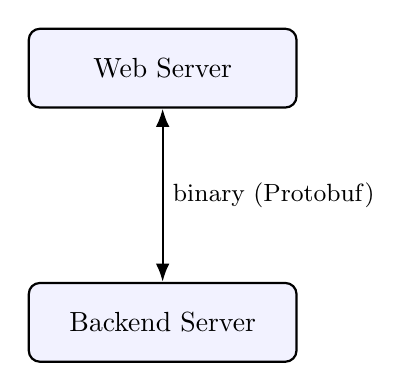
\begin{tikzpicture}[
    node distance=2.2cm, >=Latex, thick,
    box/.style={rectangle, draw, minimum width=3.4cm, minimum height=1cm,
                rounded corners, fill=blue!5}
]
  \node[box] (web)     {Web Server};
  \node[box, below=of web] (backend) {Backend Server};
  \draw[<->] (web) -- node[right] {\small binary (Protobuf)} (backend);
\end{tikzpicture}
\end{center}

The web server speaks JSON to the user and protobuf to the backend, serving as a translator between the readable and the efficient.

\subsection{Defining Messages in a \texttt{.proto} File}

Protobuf's rigour begins at its schema. Messages are declared in \texttt{.proto} files, which specify the fields, their types, and their cardinalities. Types mirror those familiar from systems languages: \texttt{double} (analogous to a C++ floating-point), \texttt{int32}, \texttt{string}, and so on.

A recurring idiom in tensor-shaped data is the \emph{shape} field, a repeated integer sequence that records the dimensions of a flattened array.

\begin{lstlisting}
message ImageClassifierInput {
  repeated int32 shape = 1;     // e.g. [height, width, channels]
  repeated double data  = 2;    // flattened pixel data
}
\end{lstlisting}

\begin{remark}
The shape field earns its keep the moment one wishes to send a colour image --- a three-dimensional array --- over a wire that understands only bytes. Without explicit dimensions, there is no way for the receiver to distinguish a $3\times 4$ matrix from a $4\times 3$ matrix from a $12$-vector. The same information then drives any \texttt{reshape} performed on the other side.
\end{remark}

% ============================================================
\section{gRPC}


\subsection{Motivation}

REST over HTTP/1.1 is universal, well-understood, and, for inter-service communication at scale, often inadequate. Its textual format inflates payloads; its request/response model leaves capacity on the table; its loose typing forces expensive parsing on the hot path. When services are geographically dispersed --- as they increasingly are --- these inefficiencies compound.

gRPC (gRPC Remote Procedure Call) is an open-source framework, originally developed at Google, that addresses these concerns head-on. It allows a program to invoke a procedure on a remote machine with nearly the syntactic ease of a local call, and it does so with a performance profile suitable for the innermost loops of a distributed system.

\subsection{The Three Pillars of gRPC}

\begin{description}
    \item[Protocol Buffers as the IDL.] The service contract --- methods, request types, response types --- is declared in a \texttt{.proto} file. Protobuf then handles serialisation, producing a compact binary on the wire.

    \item[HTTP/2 as the transport.] In contrast to HTTP/1.1, HTTP/2 provides:
    \begin{itemize}
        \item \emph{multiplexing}: many concurrent requests and responses share a single TCP connection, eliminating head-of-line blocking;
        \item \emph{header compression} via HPACK, which reduces per-message overhead;
        \item \emph{server push}, allowing the server to anticipate the client.
    \end{itemize}

    \item[Strong typing.] Unlike string-based RPC, every field in a gRPC call is typed at compile time. Specifying a \texttt{double} means exactly that; no runtime interpretation of ambiguous strings is required. The consequence is both performance (parsing is cheap, since the schema is known) and reliability (whole classes of bugs are caught before deployment).
\end{description}

\begin{remark}
A \texttt{.proto} definition is compiled, via a code generator, into idiomatic data structures for many target languages --- Python, Go, Java, C++, and others. A project-local script (e.g.\ one invoking \texttt{protoc} or a wrapper such as \texttt{rankodgen}) typically handles this step, ensuring that client and server are always in structural agreement.
\end{remark}

\subsection{Architectural Vignette: Web Server, Backend, and Peers}

Consider the following pattern of inter-service communication.

\begin{center}
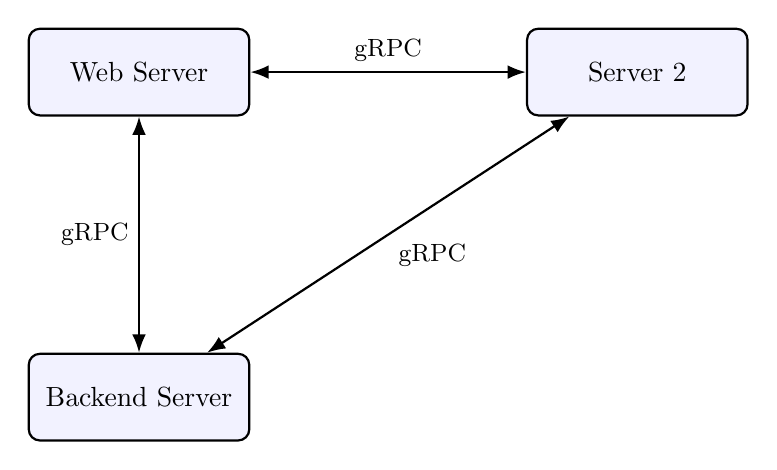
\begin{tikzpicture}[
    node distance=3cm and 3.5cm, >=Latex, thick,
    svc/.style={rectangle, draw, minimum width=2.8cm, minimum height=1.1cm,
                rounded corners, fill=blue!5}
]
  \node[svc] (web)     {Web Server};
  \node[svc, right=of web] (server2)  {Server 2};
  \node[svc, below=of web] (backend) {Backend Server};

  \draw[<->] (web)     -- node[above] {\small gRPC} (server2);
  \draw[<->] (web)     -- node[left]  {\small gRPC} (backend);
  \draw[<->] (backend) -- node[below right] {\small gRPC} (server2);
\end{tikzpicture}
\end{center}

The web server talks to both a backend server and an auxiliary service (``Server 2''); the backend, in turn, maintains its own channel to Server 2. Every edge in this graph is a strongly typed gRPC call.

% ============================================================
\section{Geography and Hardware: A Systems Aside}


The performance of a distributed system is, to a surprising degree, dictated by geography and by the nature of the hardware available in each locale.

\subsection{Regional Infrastructure and CDNs}

When a user-facing application must feel instantaneous, one does not fight the speed of light head-on; one works around it. Content Delivery Networks (\textsc{cdn}s) place frontend servers geographically close to the user, so that the first round trip is short. This works admirably for cached content and for the initial handshake, but it shifts, rather than eliminates, the problem. The regional frontend must still reach a backend --- frequently a more distant one --- to fetch dynamic data or execute business logic. That inter-service leg, typically a gRPC call, becomes the new latency budget to guard jealously.

\subsection{CPU versus GPU}

GPUs and CPUs differ not only in architecture but in their sociology of deployment.

\begin{description}
    \item[GPUs.] Specialised for parallel, compute-intensive workloads. GPU-equipped data centres are comparatively scarce, constrained by supply, by power, and increasingly by regulation. They cannot be placed arbitrarily close to users.
    \item[CPUs.] General-purpose, ubiquitous, and straightforward to rack. CPU-based capacity is available in almost any metropolitan area and is far easier to scale geographically.
\end{description}

\begin{example}[Everyday distributed systems]
\emph{YouTube} relies on globally distributed, CPU-based caching servers to deliver video at scale. \emph{Steam}'s famously high download speeds likewise reflect localised, CPU-based caches. The heavy GPU inference, where it occurs at all, is concentrated in a handful of central data centres and reached over the network.
\end{example}

\subsection{A Reference Topology}

Putting the pieces together:

\begin{center}
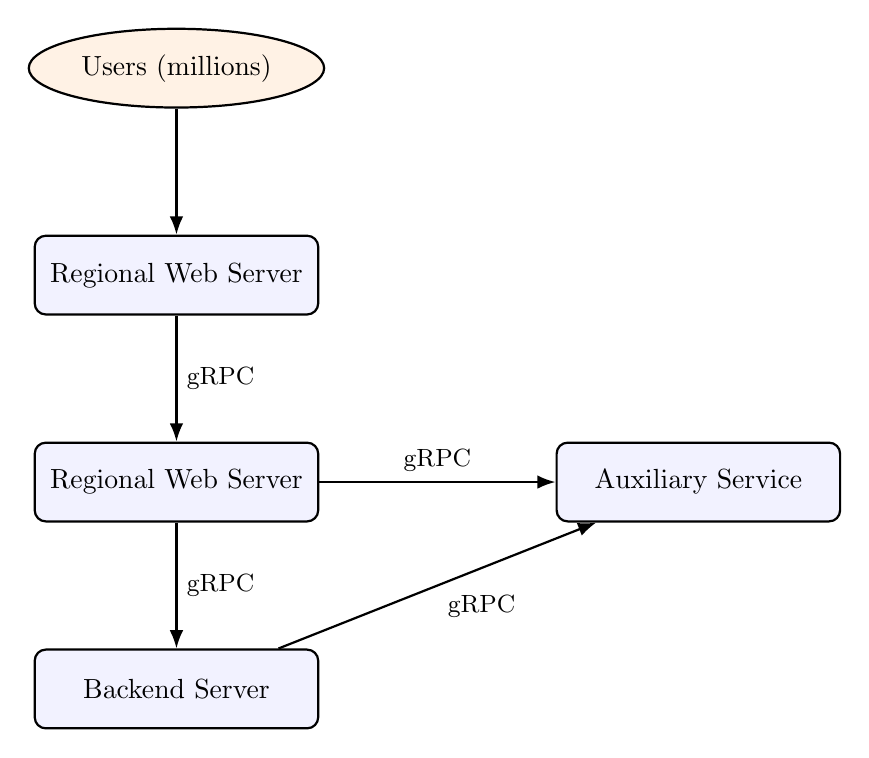
\begin{tikzpicture}[
    node distance=1.6cm, >=Latex, thick,
    box/.style={rectangle, draw, minimum width=3.6cm, minimum height=1cm,
                rounded corners, fill=blue!5},
    user/.style={ellipse, draw, minimum width=3.2cm, minimum height=1cm,
                 fill=orange!10}
]
  \node[user] (u1)   {Users (millions)};
  \node[box, below=of u1] (web1) {Regional Web Server};
  \node[box, below=of web1] (web2) {Regional Web Server};
  \node[box, below=of web2] (backend) {Backend Server};
  \node[box, right=3cm of web2] (s2)  {Auxiliary Service};

  \draw[->] (u1)   -- (web1);
  \draw[->] (web1) -- node[right]{\small gRPC} (web2);
  \draw[->] (web2) -- node[right]{\small gRPC} (backend);
  \draw[->] (web2) -- node[above]{\small gRPC} (s2);
  \draw[->] (backend) -- node[below right]{\small gRPC} (s2);
\end{tikzpicture}
\end{center}

The diagram is simplified, but its message is not: the user-facing edges are close, cheap, and plentiful; the inner edges are few, expensive, and worth optimising.

% ============================================================
\section{An Inference API Over gRPC}

We conclude by tying the two modalities --- HTTP for the edge, gRPC for the interior --- into a single coherent service.

\subsection{The Two-Layer Architecture}

\begin{center}
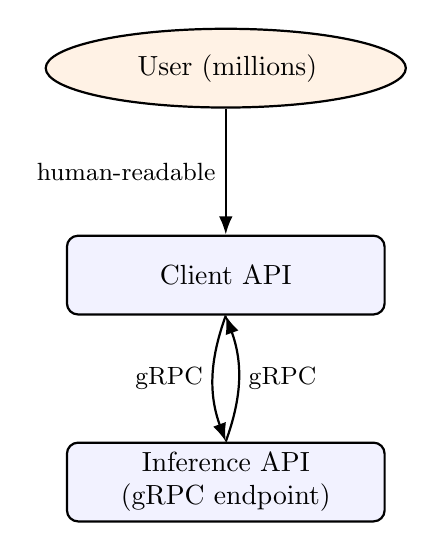
\begin{tikzpicture}[
    node distance=1.6cm, >=Latex, thick,
    box/.style={rectangle, draw, text width=3.8cm, align=center,
                minimum height=1cm, rounded corners, fill=blue!5},
    user/.style={ellipse, draw, text width=3cm, align=center,
                 minimum height=1cm, fill=orange!10}
]
  \node[user] (u) {User (millions)};
  \node[box, below=of u] (cap) {Client API};
  \node[box, below=of cap] (iap) {Inference API\\(gRPC endpoint)};

  \draw[->] (u) -- node[left]{\small human-readable} (cap);
  \draw[->] (cap.south) to[bend right=20] node[left]{\small gRPC} (iap.north);
  \draw[->] (iap.north) to[bend right=20] node[right]{\small gRPC} (cap.south);
\end{tikzpicture}
\end{center}

The \textbf{Client API} is the system's façade: it accepts human-readable requests (JSON over HTTP), handles authentication, applies business logic, and translates the request into a gRPC call to the Inference API. The \textbf{Inference API} --- the computational core --- performs the machine learning inference and returns a typed response, which the Client API then renders back into JSON for the user.

This separation is not accidental. A gRPC endpoint is not naturally user-facing: browsers prefer JSON, and the elaborate dance of translating a browser request directly into a strictly typed protobuf message is both computationally and developmentally impractical. The Client API absorbs this translation, decoupling the performant backend from the accessible frontend.

\subsection{Schemas, Shared Between Client and Server}

The Client API and the Inference API must agree, down to the last field, on the schema of their messages. The gRPC framework makes this agreement concrete through a pair of structures --- conventionally \texttt{ImageClassifierInput} and \texttt{ImageClassifierOutput} --- generated from a common \texttt{.proto} file.

\begin{remark}[Structural isomorphism]
\texttt{ImageClassifierOutput} and a related \texttt{LabelEncoding} structure may turn out to be structurally identical. This is a feature, not a coincidence: reusing a single definition in both the inference service and the client library keeps the surface area small and the maintenance cost correspondingly low. Two APIs implemented in different languages may still share, byte for byte, the same schema.
\end{remark}

If the Client API were to emit a request in a structure inconsistent with the server's expectation, the cast on the server side would fail and the request would be rejected before any inference code executed --- a failure mode that, mercifully, shows up at the first test run rather than in production.

\subsection{Server-Side Implementation Sketch}

On the server side, the inference service is exposed via a \texttt{server} function that constructs and starts a gRPC server using \texttt{grpcio}:

\begin{lstlisting}[language=Python]
from concurrent import futures
import grpc
import inference_pb2_grpc as pb2_grpc
from classifier import ImageClassifierServicer

def serve():
    server = grpc.server(futures.ThreadPoolExecutor(max_workers=10))
    pb2_grpc.add_ImageClassifierServicer_to_server(
        ImageClassifierServicer(), server
    )
    server.add_insecure_port("[::]:5051")
    server.start()
    server.wait_for_termination()
\end{lstlisting}

The generated \texttt{inference\_pb2\_grpc} module supplies the boilerplate; our \texttt{ImageClassifierServicer} supplies the logic.

\subsection{The \texttt{predict} Method}

The servicer is a subclass of the generated stub base, and the core of its implementation is the \texttt{predict} method. Within it, the request's \texttt{shape} and \texttt{data} fields are unpacked, reconstituted into a NumPy array of the correct dimensions, and passed to the model.

\begin{lstlisting}[language=Python]
import numpy as np

class ImageClassifierServicer(pb2_grpc.ImageClassifierServicer):
    def predict(self, request, context):
        array = np.array(request.data, dtype=np.float64).reshape(request.shape)
        label, confidence = self.model.infer(array)
        return pb2.ImageClassifierOutput(label=label, confidence=confidence)
\end{lstlisting}

\subsection{Client-Side Implementation Sketch}

On the client side, one opens an \emph{insecure channel} to the inference endpoint --- port 5051 in our example --- constructs a message of type \texttt{ImageClassifierInput}, and invokes the stub:

\begin{lstlisting}[language=Python]
import grpc
import inference_pb2 as pb2
import inference_pb2_grpc as pb2_grpc

def classify(array):
    channel = grpc.insecure_channel("localhost:5051")
    stub = pb2_grpc.ImageClassifierStub(channel)
    request = pb2.ImageClassifierInput(
        shape=list(array.shape),
        data=array.flatten().tolist(),
    )
    return stub.predict(request)
\end{lstlisting}

This is the whole of the plumbing. The channel transmits bytes; the stub enforces types; the protobuf messages serialise structure. Everything else --- Flask, Prometheus, Grafana, the layered JSON façade --- is arranged in concentric rings around this inner call.

% ============================================================
\section{Closing Remarks}

We have travelled a considerable distance in a short time: from the layered structure of the TCP/IP stack, through the grammar of HTTP requests and responses, into the pragmatics of deploying and monitoring a Flask service, and finally into the design of a two-tier inference API built on gRPC and Protocol Buffers.

Two themes recur. The first is the productive tension between \emph{accessibility} and \emph{efficiency}: JSON is for humans and the edges of a system; binary formats are for machines and the interior. The second is the cost of abstraction: each layer --- TCP over IP, HTTP over TCP, gRPC over HTTP/2, the Client API over gRPC --- buys convenience in exchange for overhead, and the engineer's craft lies in choosing the overhead wisely.

The forthcoming FDL module will revisit batching, caching, and tensor-graph optimisation in proper technical detail. For those of you considering entrepreneurial ventures, the framework established here is the scaffold on which a real product is built; for those of you who are merely curious, it is, I hope, a coherent account of why the web looks the way it does.

\vfill
\begin{flushright}
\textit{--- end of lecture ---}
\end{flushright}

\end{document}
